\subsubsection{IU 01: Principal} \label{iu01}
  \textbf{Objetivo} \par
  En esta vista se le permite al usaurio o sub-usuario acceder al sistema después de haber ingresando los datos requeridos para iniciar su sesión. \par
  \textbf{Diseño} \par
  Es la vista principal del sistema para el usuario o sub-usaurio a la cual se accede al abrir la aplicación móvil. Se cuentan con dos botónes que redireccionan al usuario a la vista donde podra iniciar sesión o registrarse como nuevo usuario.
    \begin{center}
      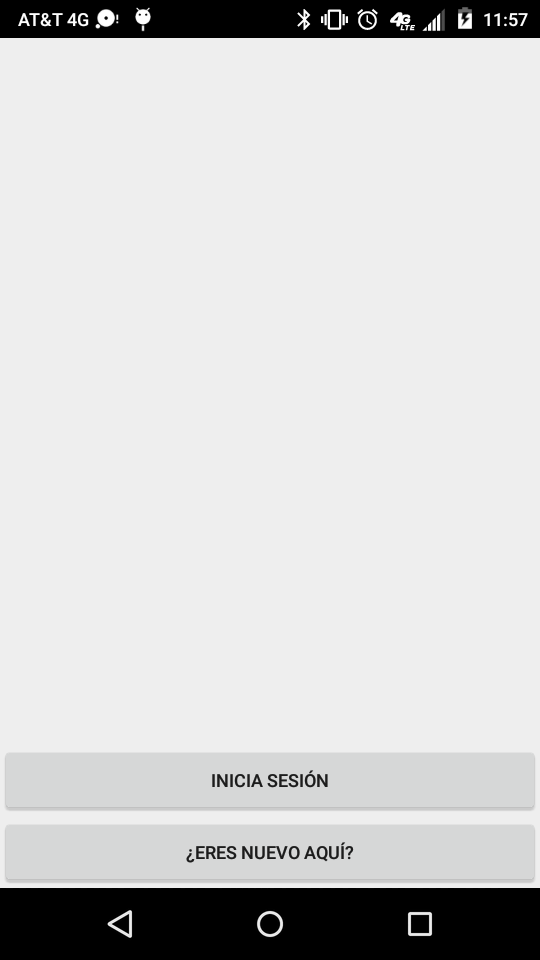
\includegraphics[scale=.2]{Capitulo3/img/gui/IU_Principal.png}
      \captionof{figure}{\nameref{iu01}}
      \label{fig:iu01_fig}
    \end{center}
  \textbf{Comandos}
    \begin{itemize}
      \item \textit{Iniciar sesión}: Muestra la vista \textbf{\nameref{iu03}} donde el usuario o sub-ususario podra ingresar al sistema.
      \item \textit{¿Eres nuevo aquí?}: Muestra la vista \textbf{\nameref{iu04}} donde el usuario podra registrarse en el sistema.
    \end{itemize}
\textbf{Mensajes} No hay mensajes que se desplieguen en esta interfaz.
  
\subsubsection{IU 03: Iniciar sesión} \label{iu03}
  \textbf{Objetivo} \par
  En esta vista se le permite al usaurio o sub-usuario acceder al sistema después de haber ingresando los datos requeridos para iniciar su sesión. \par
  \textbf{Diseño} \par
  Es la pantalla principal del sistema para el usuario o sub-usaurio a la cual se accede al abrir la aplicación móvil. Para ingresar al sistema el usuario o sub-usuario debe ingresar su correo electrónico y su contraseña en los campos de texto proporcionados. En dado caso que haya olvidado su contraseña puede seleccionar la opción de \textit{¿Olvidaste tu contraseña?} para obtener una nueva y si desea registrarse puede oprimir el botón de \textit{¿Eres nuevo aqui?}.
    \begin{center}
      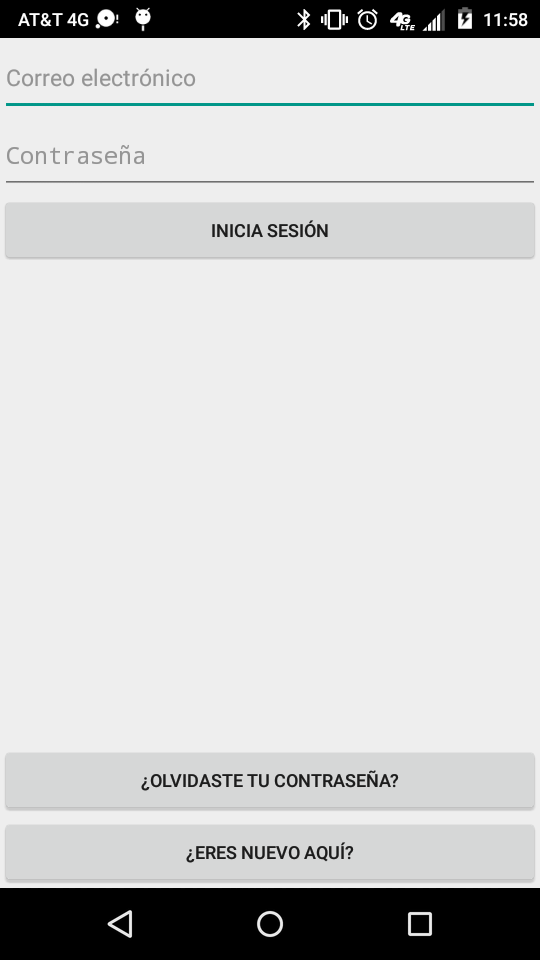
\includegraphics[scale=.2]{Capitulo3/img/gui/IU_Iniciar_sesion.png}
      \captionof{figure}{\nameref{iu03}}
      \label{fig:iu03_fig}
    \end{center}
  \textbf{Comandos}
    \begin{itemize}
      \item \textit{Iniciar sesión}: Envia una petición de acceso al sistema con los datos ingresados por el ususario.
      \item \textit{¿Olvidaste tu contraseña?}: Muestra la vista \textbf{\nameref{iu04}} donde el usuario podra registrarse en el sistema.
      \item \textit{¿Eres nuevo aquí?}: Muestra la vista \textbf{\nameref{iu05}} donde el usuario podra registrarse en el sistema.
    \end{itemize}
\textbf{Mensajes}
  \begin{itemize}
     \item \textbf{\ref{msja_01}}
     \item \textbf{\ref{msje_01}}
     \item \textbf{\ref{msje_02}}
  \end{itemize}
  
      \subsubsection{IU 04: Resetear contraseña} \label{iu04}
  \textbf{Objetivo} \par
  En esta vista el usuario puede ingresar su correo electrónico para obtener una nueva contraseña. \par
  \textbf{Diseño} \par
  En esta vista el usuario cuenta con un campo de texto donde puede ingresar su correo electrónico para solicitar una nueva contraseña que sera enviada por medio de un correo eletrónico.
    \begin{center}
      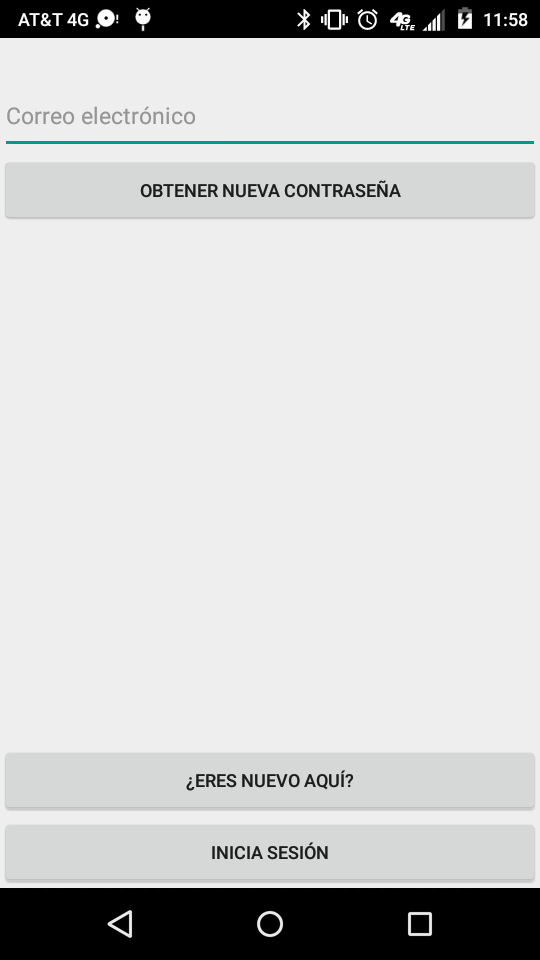
\includegraphics[scale=.2]{Capitulo3/img/gui/IU_Resetear_contrasena.png}
      \captionof{figure}{\nameref{iu04}}
      \label{fig:iu04_fig}
    \end{center}
  \textbf{Comandos}
    \begin{itemize}
      \item \textit{Obtener nueva contraseña}: Envia un petición al sistema para resetear la contraseña del usuario y enviarle un correo con la nueva contraseña que le fue asignada.
      \item \textit{¿Eres nuevo aquí?}: Muestra la vista \textbf{\nameref{iu05}} donde el usuario podra registrarse en el sistema.
      \item \textit{Iniciar sesión}: Muestra la vista \textbf{\nameref{iu03}} donde el usuario o sub-ususario podra ingresar al sistema.
    \end{itemize}
\textbf{Mensajes}
  \begin{itemize}
     \item \textbf{\ref{msja_01}}
     \item \textbf{\ref{msjn_01}}
     \item \textbf{\ref{msje_01}}
     \item \textbf{\ref{msje_02}}
  \end{itemize}
  
  
  \subsubsection{IU 05: Registrarse} \label{iu05}
  \textbf{Objetivo} \par
  En esta vista se le permite al una persona registrarse como usuario en el sistema. \par
  \textbf{Diseño} \par
  Es esta vista el usuario puede registrarse ingresando los datos que se piden en el formulario desplegado. Dependiendo del campo seran los datos que tendra que ingresar mediante el teclado o usando los selectores proporcionados. En dado caso que ya tenga una cuenta puede pulsar el botón de \textit{¿Ya tienes una cuenta?} para que se muestre la vista \textbf{\nameref{iu03}}.
    \begin{center}
      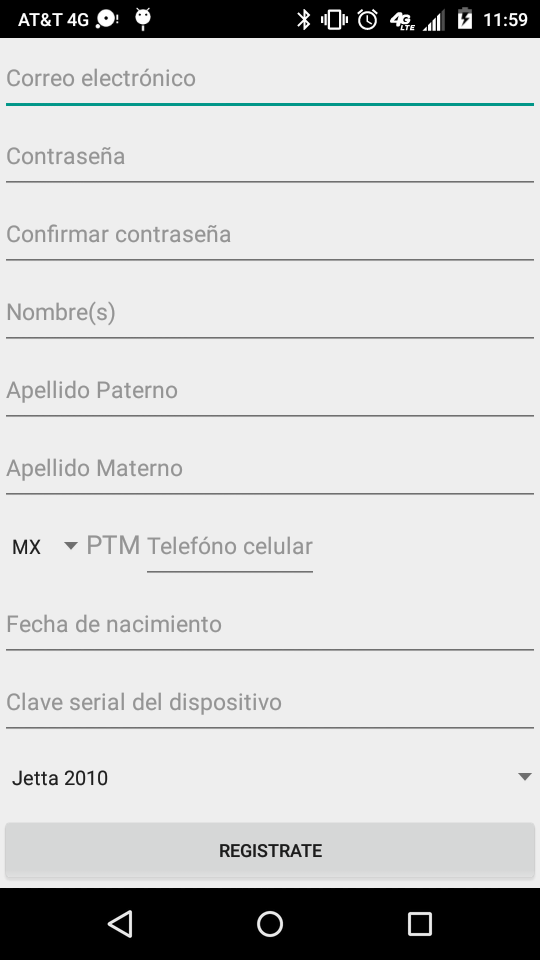
\includegraphics[scale=.2]{Capitulo3/img/gui/IU_Registrarse_(1).png}
      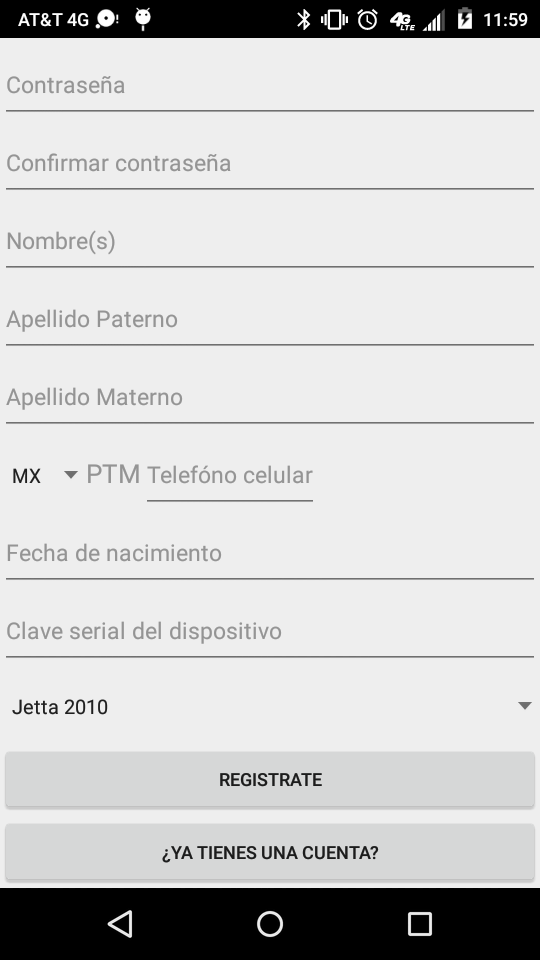
\includegraphics[scale=.2]{Capitulo3/img/gui/IU_Registrarse_(2).png}
      \captionof{figure}{\nameref{iu04}}
      \label{fig:iu05_fig}
    \end{center}
  \textbf{Comandos}
    \begin{itemize}
      \item \textit{Registrate}: Envia una petición de registro al sistema con los datos ingresados por el sistema.
      \item \textit{Iniciar sesión}: Muestra la vista \textbf{\nameref{iu03}} donde el usuario o sub-ususario podra ingresar al sistema.
    \end{itemize}
\textbf{Mensajes}
  \begin{itemize}
    \item \textbf{\ref{msja_01}}
    \item \textbf{\ref{msje_02}}
    \item \textbf{\ref{msje_03}}
    \item \textbf{\ref{msje_04}}
    \item \textbf{\ref{msje_05}}
    \item \textbf{\ref{msje_06}}
    \item \textbf{\ref{msje_07}}
    \item \textbf{\ref{msje_08}}
    \item \textbf{\ref{msjn_04}}
  \end{itemize}
  

      \subsubsection{IU 06: Confirmar teléfono} \label{iu06}
  \textbf{Objetivo} \par
  En esta vista el usuario debe ingresar el código de verificación que fue enviado al número de celular ingresado al registrarse. \par
  \textbf{Diseño} \par
  Es esta vista el usuario puede obtener una nueva contraseña ingresando su correo electrónico, al cual se le enviara la nueva contraseña. En dado caso que ya tenga una cuenta puede pulsar el botón de \textit{¿Ya tienes una cuenta?} para que se muestre la vista \textbf{\nameref{iu03}}.
    \begin{center}
      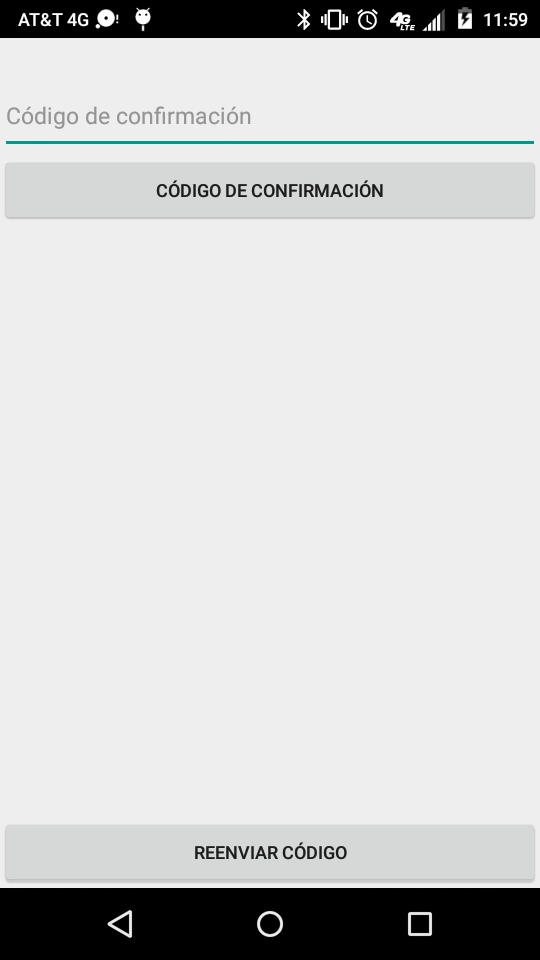
\includegraphics[scale=.2]{Capitulo3/img/gui/IU_Confirmar_telefono.png}
      \captionof{figure}{\nameref{iu04}}
      \label{fig:iu06_fig}
    \end{center}
  \textbf{Comandos}
    \begin{itemize}
      \item \textit{Código de confirmación}: Envia un petición al sistema para confirmar el teléfono verificando si el código ingresado es igual al que fue enviado.
      \item \textit{Reenviar código}: Envía una petición al sistema para mandar otro código de verificación al teléfono registrado.
    \end{itemize}
\textbf{Mensajes}
  \begin{itemize}
    \item \textbf{\ref{msja_01}}
    \item \textbf{\ref{msjc_01}}
    \item \textbf{\ref{msjn_02}}
    \item \textbf{\ref{msjn_03}}
    \item \textbf{\ref{msje_09}}
  \end{itemize}